% There will be a graph in here.
\section{Graphs}
\label{sec:Graph}
A graph will go below here.

First a slight change here.

And another small change.

\begin{knitrout}
\definecolor{shadecolor}{rgb}{1, 1, 1}\color{fgcolor}\begin{kframe}
\begin{flushleft}
\ttfamily\noindent
\hlfunctioncall{plot}\hlkeyword{(}\hlnumber{1}\hlkeyword{:}\hlnumber{10}\hlkeyword{,}{\ }\hlnumber{1}\hlkeyword{:}\hlnumber{10}\hlkeyword{)}\mbox{}
\normalfont
\end{flushleft}
\end{kframe}\begin{figure}[!hbtp]


{\centering 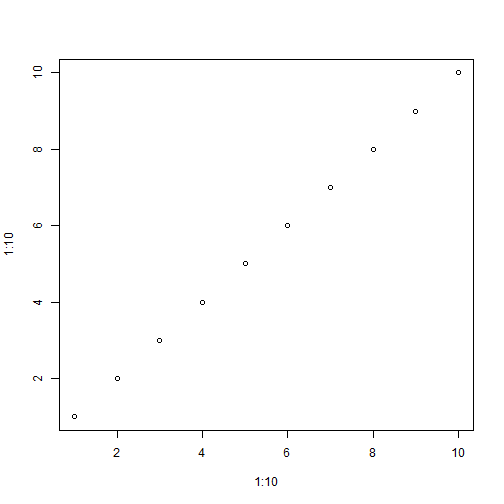
\includegraphics[width=.45\linewidth]{chunk2/figure/first-plot} 

}

\caption[First Graph]{The first graph of this one.\label{fig:first-plot}}
\end{figure}

\end{knitrout}


And then some more stuff.

And a bit more.
